\section{Simulation}

In this section, the simulations of the LNA and the corresponding matching networks will be presented.

\subsection{Validation of the LNA design}

First, using the LTSpice, the T502 transistor was added and the parasites capacitance and inductance of the package were considered, resulting in the simulated real transistor circuit in Figure \ref{fig:TransistorReal}.

\begin{figure}[H]
    \centering
    \includegraphics*[scale = 0.3]{Images/TransistorReal.png}
    \caption{Transistor with package effects}
    \label{fig:TransistorReal}
\end{figure}

After this, the biasing circuit of the transistor for the required  parameters is present in Figure \ref{fig:SIMBiasCircuit}.
\textcolor{red}{explicar a existencia de bobinas e condensadores}

\begin{figure}[H]
    \centering
    \includegraphics*[scale = 0.3]{Images/SIMBiasCircuit.png}
    \caption{Biasing circuit simulated}
    \label{fig:SIMBiasCircuit}
\end{figure}

After simulating the operation point of the previous circuit, the result for the required parameters is shown in Figure \ref{fig:SIMBias}.

\begin{figure}[H]
    \centering
    \includegraphics*[scale = 0.3]{Images/SIMBias.png}
    \caption{Result of the operation point simulation}
    \label{fig:SIMBias}
\end{figure}

After analyzing the previous graphic, it is possible to confirm that result parameters of the biasing circuit are within the required.

At the same time, the same circuit was implemented in Cadence, to ensure greater reliability of the results obtained. So, this circuit can be seen in Figure \ref{fig:CadenceBiasCircuit}.

\begin{figure}[H]
    \centering
    \includegraphics*[scale = 0.1]{Images/CadenceBiascircuit.png}
    \caption{Biasing circuit simulated in Cadence}
    \label{fig:CadenceBiasCircuitBiasCircuit}
\end{figure}

So the matching networks for the source and the load, both with an impedance of $50\Omega$, can be implemented.

\subsection{Input and output matching networks design simulation} 

As mentioned before, the first step in designing a matching network in an LNA is to know the S-parameters of the amplifier circuit, so, switching to an AC analysis of the LNA circuit, and adding both the source and the load, the simulated circuit is shown in Figure \ref{fig:SIMS-paramCircuit}.

\begin{figure}[H]
    \centering
    \includegraphics*[scale = 0.3]{Images/S-paramCircuit.png}
    \caption{Circuit for the S-parameters}
    \label{fig:SIMS-paramCircuit}
\end{figure}

The resulting S-parameters can be seen in Figure \ref{fig:SimS-param}.

\begin{figure}[H]
    \centering
    \begin{subfigure}{0.4\textwidth}
        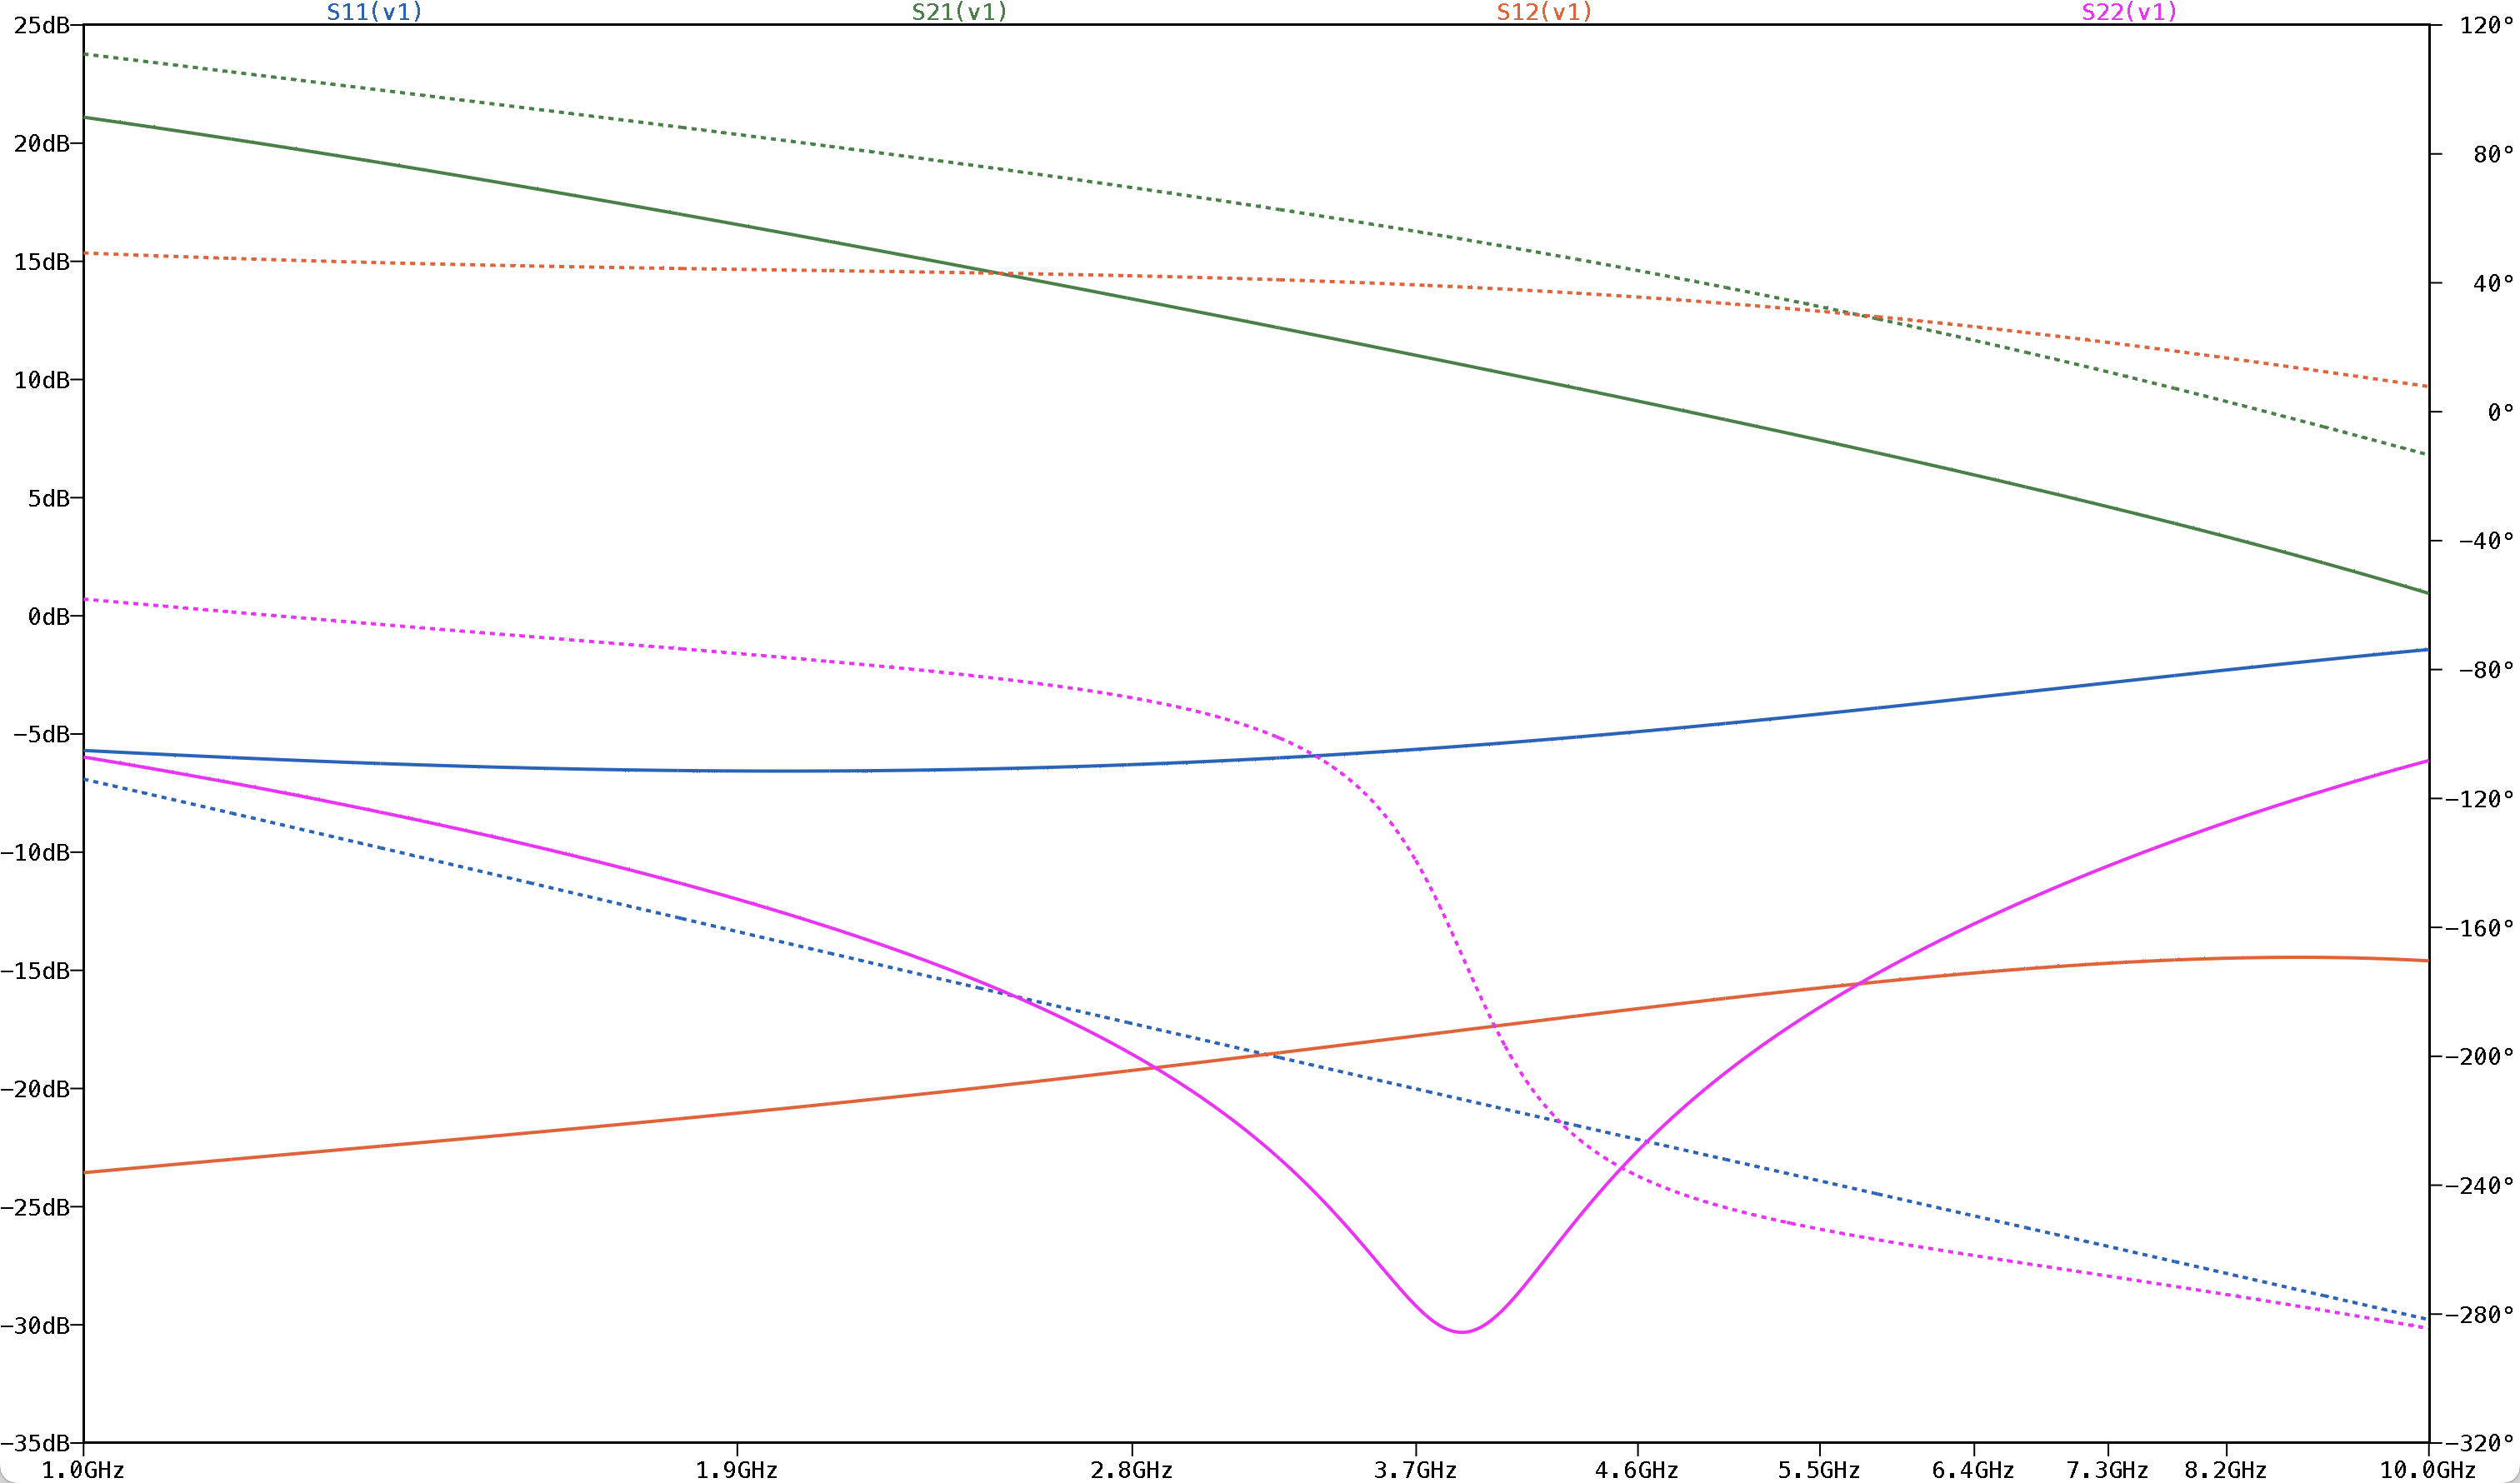
\includegraphics[width=1\textwidth]{Images/S-paramdB.png}
        \caption{S-parameters in dB}
    \end{subfigure}
    \hfill
    \begin{subfigure}{0.4\textwidth}
        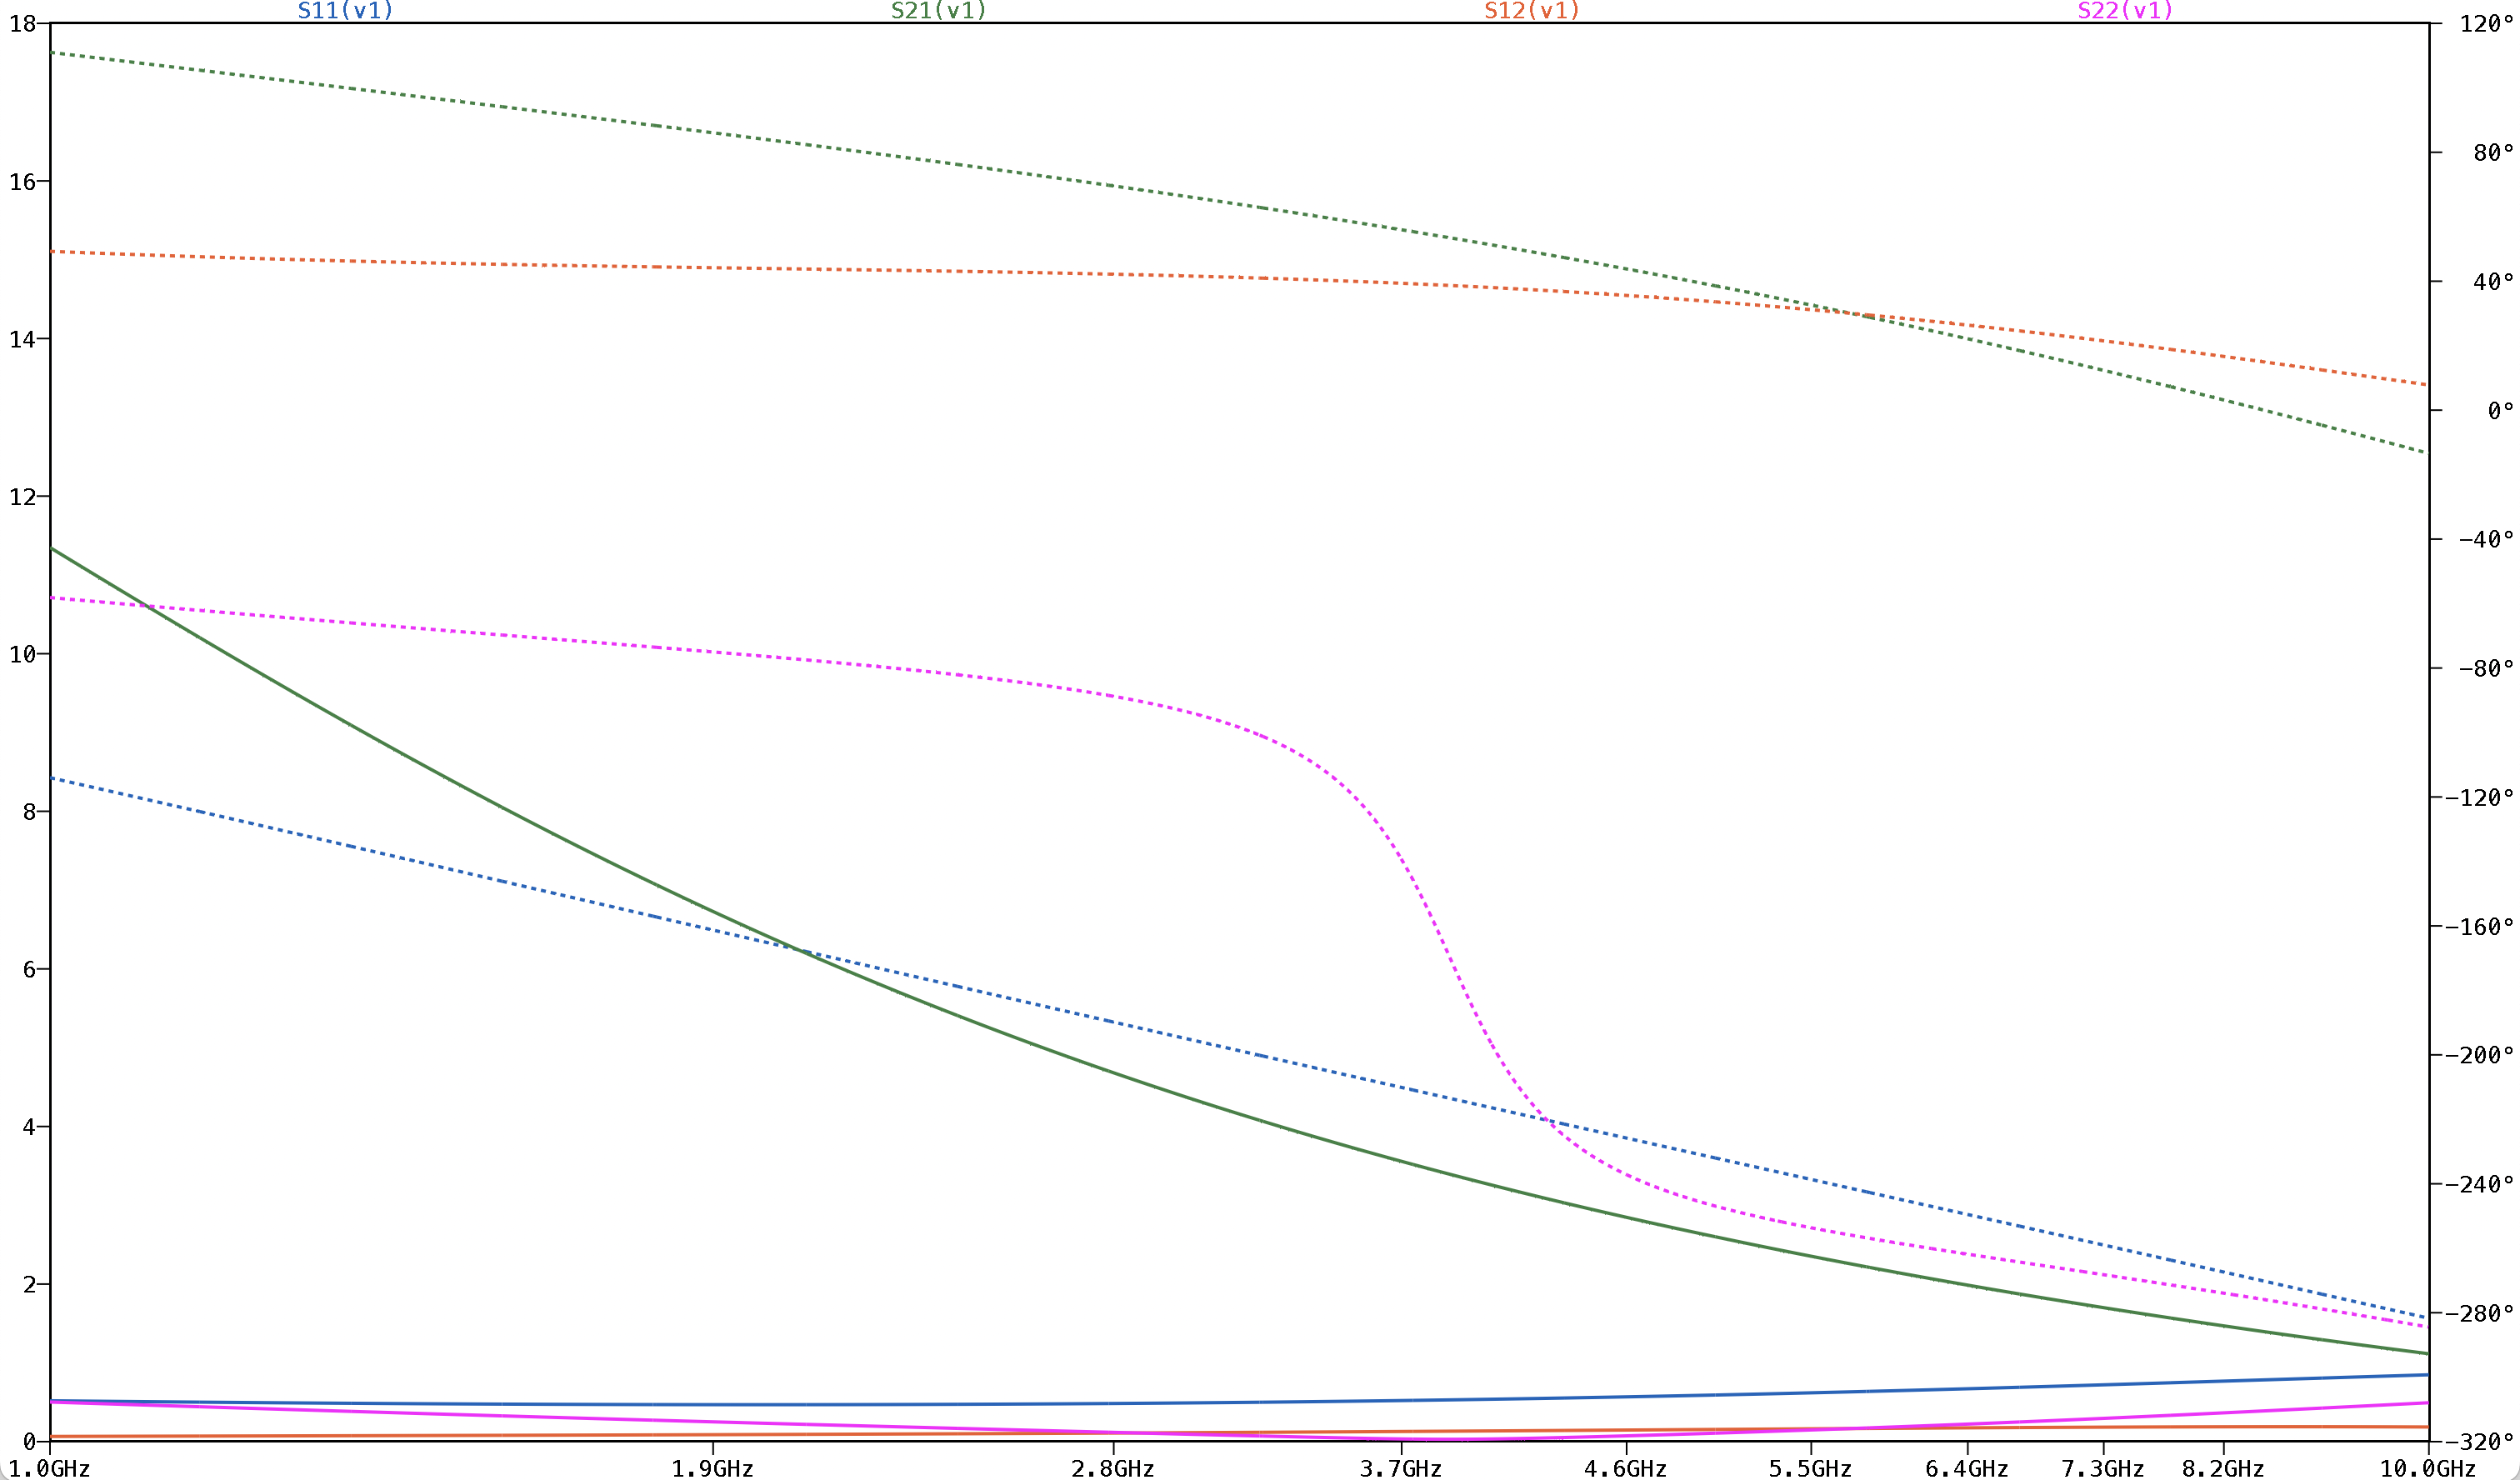
\includegraphics[width=1\textwidth]{Images/S-paramLin.png}
        \caption{S-parameters in linear}
    \end{subfigure}
    \caption{S-parameters of the LNA}
    \label{fig:SimS-param}
\end{figure}

After assuming a working frequency of $4 GHz$, the resulting matching networks using capacitors and inductors is exhibit in Figure \ref{fig:SIMLCMatchingCircuit}.

\begin{figure}[H]
    \centering
    \includegraphics*[scale = 0.3]{Images/SIMLCmatchingcircuit.png}
    \caption{Matching networks using inductors and capacitors}
    \label{fig:SIMLCMatchingCircuit}
\end{figure}

Using again the same AC analysis, the S-parameters of new circuit using the capacitors and inductors matching networks is displayed in Figure \ref{fig:SIMLCMatching}.

\begin{figure}[H]
    \centering
    \includegraphics*[scale = 0.3]{Images/SIMLCmatching.png}
    \caption{S-parameters for the matching networks using inductors and capacitors}
    \label{fig:SIMLCMatching}
\end{figure}

After looking at the graphic above, it is possible to conclude that this matching network is working properly, since there is a sharp drop in both $S11$ and $S22$ ate the desired frequency of $4GHz$ as well as a high point in the $S21$ curve.

In cadence, the circuit for the matching using inductors and capacitors is the following.

\begin{figure}[H]
    \centering
    \includegraphics*[scale = 0.1]{Images/CadenceLCcircuit.png}
    \caption{Matching networks using inductors and capacitors in Cadence}
    \label{fig:CadenceLCcircuit}
\end{figure}

Simulating, the S-parameters of this circuit with the mentioned matching networks is visible in Figure \ref{fig:CadenceLC}.

\begin{figure}[H]
    \centering
    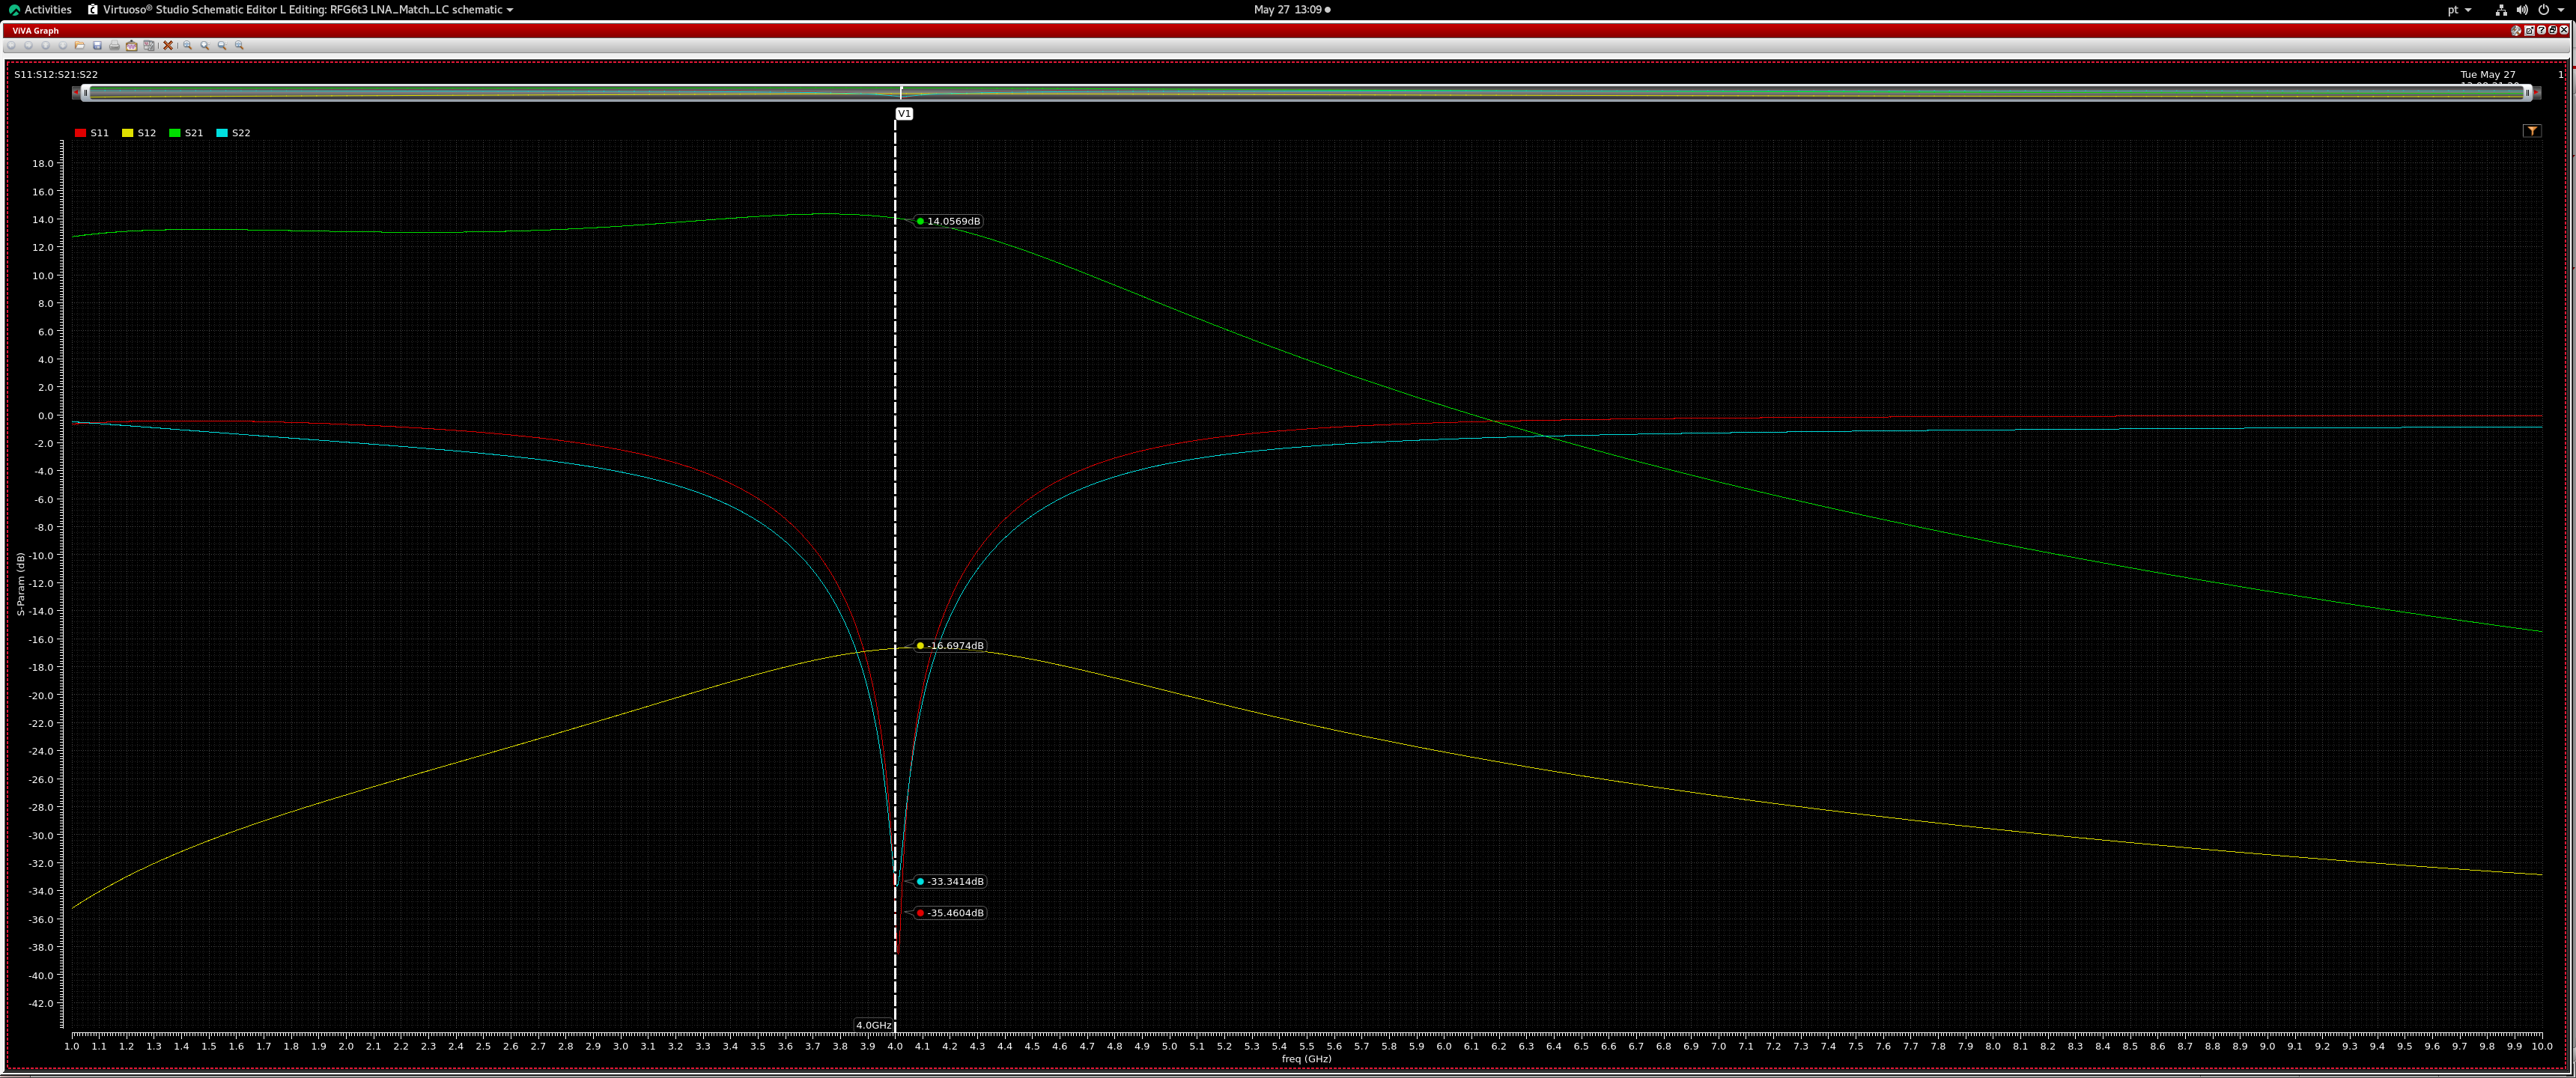
\includegraphics[width=1\textwidth]{Images/LC_matching.png}
    \caption{S-parameters for the matching networks using inductors and capacitors in Cadence}
    \label{fig:CadenceLC}
\end{figure}

Passing to the matching networks using transmission lines and stubs, and using the same working frequency, the new LNA circuit is shown in Figure \ref{fig:SIMLSMatchingCircuit}.

\begin{figure}[H]
    \centering
    \includegraphics*[scale = 0.3]{Images/SIMLSmatchingcircuit.png}
    \caption{Matching networks using transmission lines and stubs}
    \label{fig:SIMLSMatchingCircuit}
\end{figure}

The S-parameters for this new matched circuit can be seen in Figure \ref{fig:SIMLSMatching}.

\begin{figure}[H]
    \centering
    \includegraphics*[scale = 0.3]{Images/SIMLSmatching.png}
    \caption{S-parameters for the matching networks using transmission lines and stubs}
    \label{fig:SIMLSMatching}
\end{figure}

Similarly to the first matching networks, the drop in both $S11$ and $S22$ can also be seen, as well as the same approximated value of $S21$, so, this matching network using transmission lines and stubs is correctly working. 

In cadence, the circuit for the matching using transmission lines and stubs is the following.

\begin{figure}[H]
    \centering
    \includegraphics*[scale = 0.1]{Images/CadenceLScircuit.png}
    \caption{Matching networks using transmission lines and stubs in Cadence}
    \label{fig:CadenceLCcircuit}
\end{figure}

Simulating, the S-parameters of this circuit with the mentioned matching networks is visible in Figure \ref{fig:CadenceLS}.

% \begin{figure}[H]
%     \centering
%     \includegraphics*[scale = 0.3]{Images/LS_matching.png}
%     \caption{S-parameters for the matching networks using transmission lines and stubs in Cadence}
%     \label{fig:CadenceLS}
% \end{figure}

\subsection{Noise}

To simulate the noise of each matching network, the Cadence was used, resulting in the graphic shown in Figure \ref{fig:NoiseLC} for the inductors and capacitors.

\begin{figure}[H]
    \centering
    \includegraphics*[scale = 0.3]{Images/noiseLC.png}
    \caption{Noise for the matching networks using capacitors and inductors in Cadence}
    \label{fig:NoiseLC}
\end{figure}

And for transmission lines and stubs in Figure \ref{fig:NoiseLS}.

\begin{figure}[H]
    \centering
    \includegraphics*[scale = 0.3]{Images/noiseLS.png}
    \caption{Noise for the matching networks using transmission lines and stubs in Cadence}
    \label{fig:NoiseLS}
\end{figure}